%%%%%%%%%%%%%%%%%%%%%%%%%%%%%%%%%%%%%%%
% Deedy - One Page Two Column Resume
% LaTeX Template
% Version 1.2 (16/9/2014)
%
% Original author:
% Debarghya Das (http://debarghyadas.com)
%
% Original repository:
% https://github.com/deedydas/Deedy-Resume
%
% IMPORTANT: THIS TEMPLATE NEEDS TO BE COMPILED WITH XeLaTeX
%
% This template uses several fonts not included with Windows/Linux by
% default. If you get compilation errors saying a font is missing, find the line
% on which the font is used and either change it to a font included with your
% operating system or comment the line out to use the default font.
%
%%%%%%%%%%%%%%%%%%%%%%%%%%%%%%%%%%%%%%
%
% TODO:
% 1. Integrate biber/bibtex for article citation under publications.
% 2. Figure out a smoother way for the document to flow onto the next page.
% 3. Add styling information for a "Projects/Hacks" section.
% 4. Add location/address information
% 5. Merge OpenFont and MacFonts as a single sty with options.
%
%%%%%%%%%%%%%%%%%%%%%%%%%%%%%%%%%%%%%%
%
% CHANGELOG:
% v1.1:
% 1. Fixed several compilation bugs with \renewcommand
% 2. Got Open-source fonts (Windows/Linux support)
% 3. Added Last Updated
% 4. Move Title styling into .sty
% 5. Commented .sty file.
%
%%%%%%%%%%%%%%%%%%%%%%%%%%%%%%%%%%%%%%%
%
% Known Issues:
% 1. Overflows onto second page if any column's contents are more than the
% vertical limit
% 2. Hacky space on the first bullet point on the second column.
%
%%%%%%%%%%%%%%%%%%%%%%%%%%%%%%%%%%%%%%


\documentclass[]{deedy-resume-openfont}
\usepackage{fancyhdr}
\usepackage{graphicx}
\usepackage{paracol}
\usepackage{fontawesome5}
\usepackage{lastpage}
\geometry{bottom=1.5cm}
\columnratio{0.30}
\setlength{\columnsep}{0.04\textwidth}
\globalcounter{*}

\pagestyle{fancy}
\fancyhf{}
\fancyfoot[C]{\color{headings}\thepage/\pageref{LastPage}}

\begin{document}
\color{primary}
\thispagestyle{fancy}

%%%%%%%%%%%%%%%%%%%%%%%%%%%%%%%%%%%%%%
%
%     LAST UPDATED DATE
%
%%%%%%%%%%%%%%%%%%%%%%%%%%%%%%%%%%%%%%
\lastupdated

%%%%%%%%%%%%%%%%%%%%%%%%%%%%%%%%%%%%%%
%
%     CUSTOM HEADER (三栏：照片 | 姓名 | 联系方式)
%
%%%%%%%%%%%%%%%%%%%%%%%%%%%%%%%%%%%%%%
{
\noindent
\begin{minipage}[c]{0.15\textwidth}
    \centering
    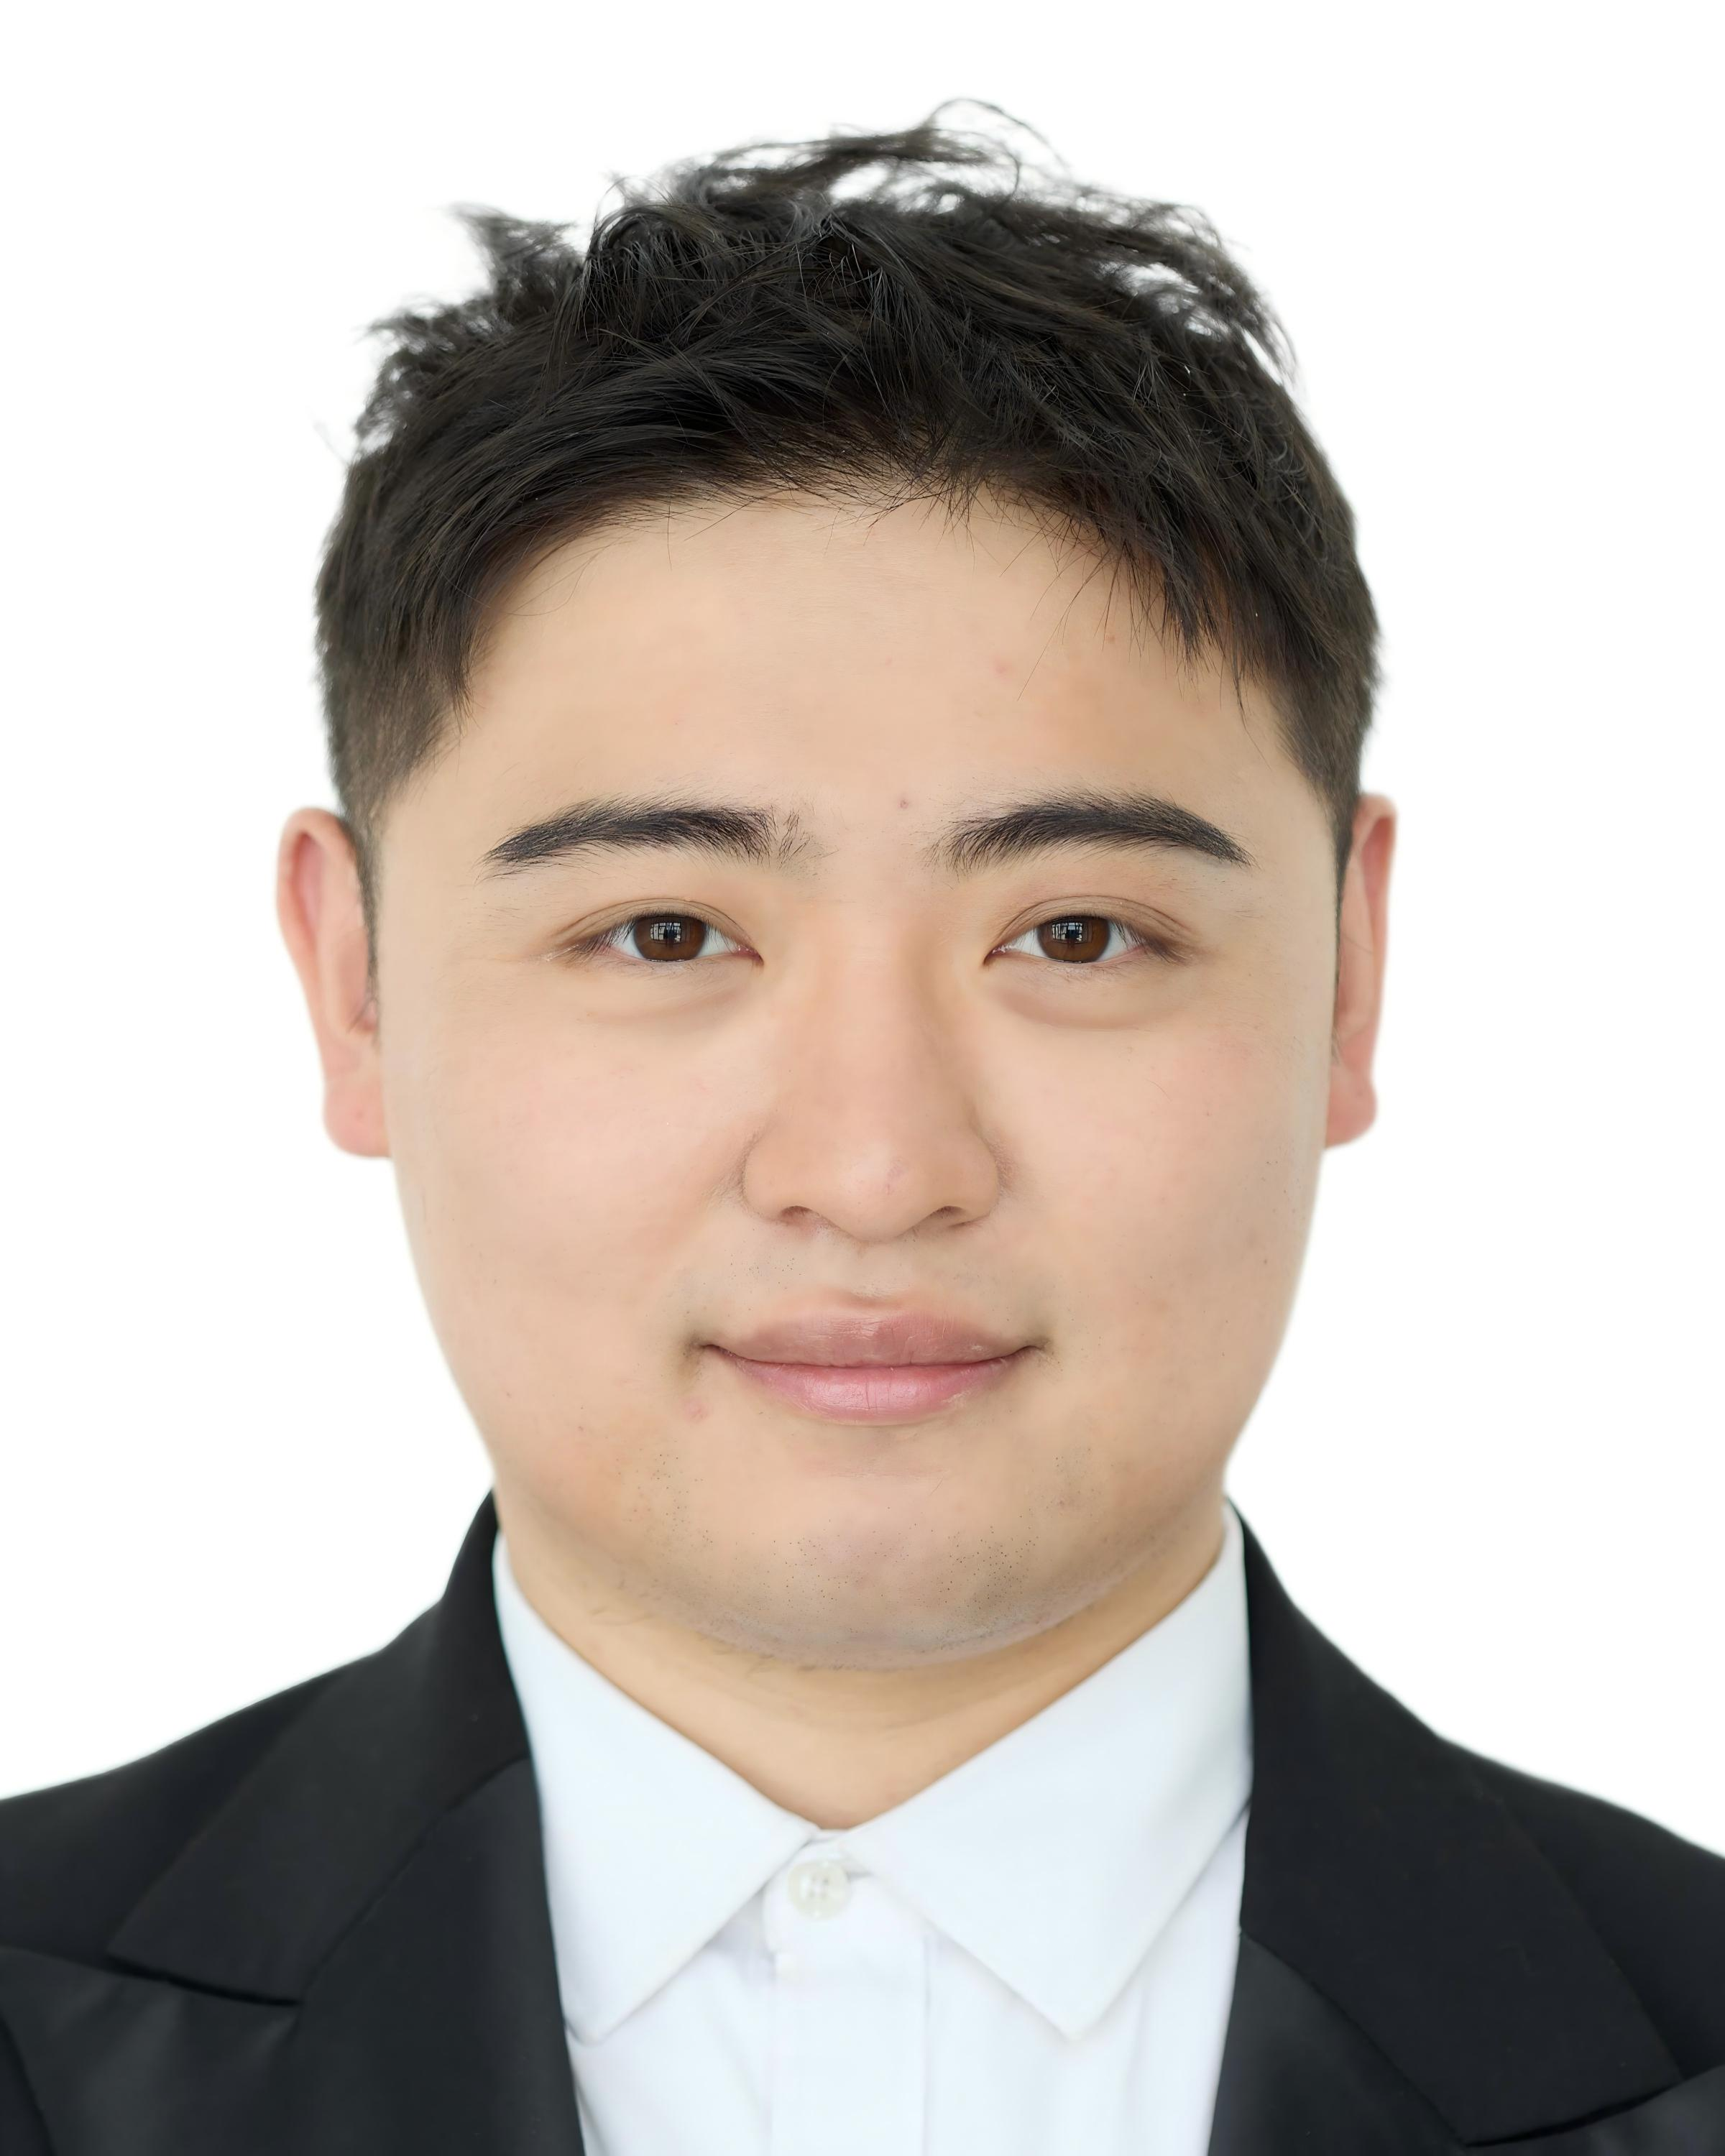
\includegraphics[height=2.2cm]{张靖昊照片.jpg}
\end{minipage}%
\hfill
\begin{minipage}[c]{0.52\textwidth}
    \centering
    {\color{primary}\fontspec[Path = fonts/, Extension=.otf, AutoFakeBold=2.5]{FZYouSong GBK}\fontsize{30pt}{30pt}\selectfont 张靖昊}
    \\[2pt]
    {\color{headings}\fontspec[Path = fonts/, Extension=.otf]{FZYouSong GBK}\fontsize{12pt}{12pt}\selectfont ZHANG Jinghao}
\end{minipage}%
\hfill
\begin{minipage}[c]{0.28\textwidth}
    \raggedright
    \color{primary}
    {\fontspec[Path = fonts/, Extension=.otf, AutoFakeBold=1.5]{FZYouSong GBK}\fontsize{10pt}{14pt}\selectfont
    {\faMapMarker*\ 浙江杭州} \\
    {\faCalendar*\ 1997} \\
    {\faEnvelope}\ \href{mailto:zhang.jing.hao@outlook.com}{zhang.jing.hao@outlook.com} \\
    {\faPhone*\ 18645858867}}
\end{minipage}
\\[5pt]
\noindent\makebox[\linewidth]{\color{accent}\rule{\paperwidth}{0.4pt}}
\vspace{-15pt}
}

%%%%%%%%%%%%%%%%%%%%%%%%%%%%%%%%%%%%%%
%
%     COLUMN ONE
%
%%%%%%%%%%%%%%%%%%%%%%%%%%%%%%%%%%%%%%

\begin{paracol}{2}
\raggedright

%%%%%%%%%%%%%%%%%%%%%%%%%%%%%%%%%%%%%%
%     EDUCATION
%%%%%%%%%%%%%%%%%%%%%%%%%%%%%%%%%%%%%%

\section{教育经历}

\subsection{悉尼科技大学}
\descript{University of Technology, Sydney}
\descript{软件工程（本科）}
\location{2017.10 - 2019.10}

\sectionsep

\subsection{哈尔滨工程大学}
\descript{Harbin Engineering University}
\descript{计算机科学与技术（本科）}
\location{2015.08 - 2019.07}

\sectionsep

%%%%%%%%%%%%%%%%%%%%%%%%%%%%%%%%%%%%%%
%     LINKS
%%%%%%%%%%%%%%%%%%%%%%%%%%%%%%%%%%%%%%

% \section{链接}
% \sectionsep
% Gitee: \href{https://gitee.com/ZBeeeeeeeeee}{https://gitee.com/ZBeeeeeeeeee} \\
% GitHub: \href{https://github.com/zbeeeeeeeeee}{https://github.com/zbeeeeeeeeee} \\

%%%%%%%%%%%%%%%%%%%%%%%%%%%%%%%%%%%%%%
%     COURSEWORK
%%%%%%%%%%%%%%%%%%%%%%%%%%%%%%%%%%%%%%

% \section{修读课程}
% \subsection{Graduate}
% Advanced Machine Learning \\
% Open Source Software Engineering \\
% Advanced Interactive Graphics \\
% Compilers + Practicum \\
% Cloud Computing \\
% Evolutionary Computation \\
% Defending Computer Networks \\
% Machine Learning \\
% \sectionsep

%%%%%%%%%%%%%%%%%%%%%%%%%%%%%%%%%%%%%%
%     SKILLS
%%%%%%%%%%%%%%%%%%%%%%%%%%%%%%%%%%%%%%

\section{技能}

\subsection{AI 智能体}
Agent \textbullet{} 多 Agent 架构 \textbullet{} MCP \textbullet{} RAG \textbullet{} Skills \textbullet{} Function Calling \textbullet{} YOLO \textbullet{} OpenCV \textbullet{} 模型微调/量化/边缘部署 \\
\sectionsep

\subsection{应用开发}
鸿蒙（ArkTS）\textbullet{} Android（Java/Kotlin）\textbullet{} Flutter \textbullet{} Vue \textbullet{} Electron \\
\sectionsep

\subsection{嵌入式}
OpenHarmony \textbullet{} STM32 \textbullet{} GPIO \textbullet{} I2C \textbullet{} UART \textbullet{} MQTT \textbullet{} 传感器驱动 \textbullet{} 网络通信 \\
\sectionsep

\subsection{软件架构 \& 后端}
\textbf{软件架构设计} \textbullet{} 微服务 \textbullet{} Java \textbullet{} Spring Boot \textbullet{} Node.js \textbullet{} RESTful API \textbullet{} MySQL \textbullet{} PostgreSQL \\
\sectionsep


%%%%%%%%%%%%%%%%%%%%%%%%%%%%%%%%%%%%%%
%     AWARDS
%%%%%%%%%%%%%%%%%%%%%%%%%%%%%%%%%%%%%%

\section{所获荣誉}

\begin{tabular}{@{}p{2em} p{\dimexpr\linewidth-2em-2\tabcolsep\relax}@{}}
\textbf{2025} & 金牌个人奖 \\[8pt]
\textbf{2025} & 华为 LCS 第一届 AI 应用开发大赛 TOP1 \\[8pt]
\textbf{2023} & 浙江华为第七届最优秀讲师大赛 TOP1 \\[8pt]
\textbf{2022} & 金牌个人奖 \\[8pt]
\textbf{2017} & 全美大学生数学建模大赛 Outstanding 奖 \\
\end{tabular}

\sectionsep

%%%%%%%%%%%%%%%%%%%%%%%%%%%%%%%%%%%%%%
%     LANGUAGES
%%%%%%%%%%%%%%%%%%%%%%%%%%%%%%%%%%%%%%

\section{语言能力}

英文可交流，可作为工作语言

IELTS 6.5 \textbullet{} 全英文跨国项目交付

\sectionsep

%%%%%%%%%%%%%%%%%%%%%%%%%%%%%%%%%%%%%%
%     LINKS
%%%%%%%%%%%%%%%%%%%%%%%%%%%%%%%%%%%%%%

\section{链接}

\href{https://gitee.com/ZBeeeeeeeeee}{Gitee: https://gitee.com/ZBeeeeeeeeee} \\
\href{https://github.com/zbeeeeeeeeee}{GitHub: https://github.com/zbeeeeeeeeee}

%%%%%%%%%%%%%%%%%%%%%%%%%%%%%%%%%%%%%%
%
%
%     COLUMN TWO
%
%%%%%%%%%%%%%%%%%%%%%%%%%%%%%%%%%%%%%%

\switchcolumn
\raggedright
\color{primary}

%%%%%%%%%%%%%%%%%%%%%%%%%%%%%%%%%%%%%%
%     EXPERIENCE
%%%%%%%%%%%%%%%%%%%%%%%%%%%%%%%%%%%%%%

\section{工作经历}

\runsubsection{浙江华为通信技术有限公司}
\descript{AI Agent 架构师 | 金牌讲师}
\location{2021.01 - 至今 | 杭州}
\begin{tightemize}
    \item 主导内部\textbf{AI Agent Harness} 平台建设，抽象 Agent 生命周期、工具调用、会话管理等通用能力，支撑多业务线智能体应用标准化接入与交付
    \item 作为公司\textbf{金牌讲师}，承担多个头部客户的培训任务，多次对接重点客户沟通需求，主导多门培训课程的设计与开发
    \item 跨团队协作推进项目交付，承担多个重点项目PM及TD角色，具备较强的项目管理与技术沟通能力
\end{tightemize}
\sectionsep

\runsubsection{同花顺}
\descript{移动应用开发工程师}
\location{2019.10 - 2020.12 | 杭州}
\begin{tightemize}
    \item 负责手机炒股 App 核心交易模块的设计与开发，支撑千万级用户交易场景
    \item 主导 AI 语音交易功能落地，参与移动端性能优化与架构迭代
\end{tightemize}
\sectionsep

%%%%%%%%%%%%%%%%%%%%%%%%%%%%%%%%%%%%%%
%     RESEARCH
%%%%%%%%%%%%%%%%%%%%%%%%%%%%%%%%%%%%%%

\section{研发项目经历}

\runsubsection{基于 AI Harness 的 HarmonyOS 辅助应用研发平台}
\descript{架构师}
\location{2026.03 - 2026.07}
\begin{tightemize}
    \item 基于 AI LLM 构建 Harness，实现从需求分析→方案制定→评审→代码编写→集成编译测试→Code Review→Git 合并→应用落地的全流程 AI 辅助研发
    \item 集成各类 CLI 工具实现 CI/CD 自动化流水线，结合 RAG 与知识图谱挂载研发垂域知识，提升研发效率与代码质量
\end{tightemize}
\sectionsep

\runsubsection{交通事故检测系统（多智能体、端边云协同）}
\descript{架构设计 \& 核心开发}
\location{2025.06 - 2026.06}
\begin{tightemize}
    \item 设计\textbf{多智能体协作管线}（场景感知→严重度评估→RAG 责任判定→报告生成），集成 MCP 协议工具调用与交通法规知识库，实现事故端到端自动分析定责
    \item 基于昇腾 310B 部署 YOLOv11 边缘推理，通过\textbf{AIPP 算子}将图像预处理卸载至 NPU，降低 CPU 负载与推理延迟
    \item 基于海思3861芯片设计鸿蒙硬件开发板并驱动传感器及周边外设，并开发鸿蒙终端应用。通过标定算法实现二维视觉坐标到经纬度映射，位置信息直传后台。
\end{tightemize}
\sectionsep

\runsubsection{OpenWork — AI Agent Harness \& 智能工作助手}
\descript{Harness 架构设计 \& 全栈开发}
\location{2026.03 - 2026.06 | 个人项目}
\begin{tightemize}
    \item 自研\textbf{AI Agent Harness}，实现 Agent 生命周期管理、多轮工具调用循环与任务编排，基于 XML 标签解析替代 JSON Function Calling，支持 OpenAI 兼容协议与流式响应，支持 MCP、Skills、RAG
    \item 设计\textbf{Skills 插件系统}与滑动窗口会话记忆，实现技能热加载与上下文动态注入；内置权限分级与沙箱隔离机制，保障工具调用安全可控
    \item 基于 Vue 3 + Monaco Editor + Electron 构建四包单体仓库桌面应用，设计三合一文件系统抽象层，支持 Server Web/桌面双模式部署
\end{tightemize}
\sectionsep

\runsubsection{基于 AI 大模型 MCP 的鸿蒙煤矿巡检机器人}
\descript{硬件设计 \& 系统开发}
\location{2025.03 - 2026.03 | 校企合作 }
\begin{tightemize}
    \item 设计巡检机器人\textbf{鸿蒙硬件系统}，集成激光雷达、红外热成像、多气体传感器、9轴IMU等感知模块，完成底盘驱动控制与开发板选型搭建
    \item 基于\textbf{鸿蒙分布式软总线}构建井下设备互联，通过 MCP 协议实现多源传感器统一接入与\textbf{自然语言控制}，探索具身智能在工业场景落地
    \item 结合华为云 IoTDA 实现端侧数据采集与平台命令下发，打通端-边-云全链路
\end{tightemize}
\sectionsep

\runsubsection{SlideGenius 帧帧成课}
\descript{AI 应用开发}
\location{2025.02 - 2025.05 | 华为内部工具}
\begin{tightemize}
    \item 基于 PPT 智能构建讲义与课程视频的自动化工具，结合数字人与 TTS 模型实现快速课程生成
    \item 设计\textbf{双智能体管线}：内容识别智能体将 PPT 切片为图片并通过 Qwen3-VL 视觉模型提取课件内容与逻辑；讲义生成智能体使用DeepSeek-V3模型构建讲义脚本，并通过上下文工程确保页间承上启下
    \item 集成数字人驱动与 TTS 语音合成，实现从 PPT 到课程视频的端到端自动生成
\end{tightemize}
\sectionsep

\runsubsection{基于 YOLO 与 STM32 的 AGV 自主循迹平台}
\descript{嵌入式 \& 视觉系统开发}
\location{2024.03 - 2024.09 | 华为}
\begin{tightemize}
    \item 设计\textbf{STM32 + CAN 总线}运动控制方案，通过 CAN 连接昇腾 310B 主控板，实现两芯片间实时指令通信与电机/舵机闭环驱动
    \item 在昇腾 310B 部署 YOLO 视觉推理，识别路面引导线与标识物，实现 AGV \textbf{自主循迹}与\textbf{运动跟随}功能
    \item 完成从硬件选型、运动控制算法、YOLO模型训练到模块集成的全链路开发，AGV 实现稳定自主行驶
\end{tightemize}
\sectionsep

\runsubsection{HCIA/HCIP 鸿蒙应用与设备认证项目}
\descript{认证架构设计 \& 鸿蒙应用 \& 嵌入式}
\location{2021.03 - 2023.06 | 华为}
\begin{tightemize}
    \item 主导鸿蒙四大认证体系（HCIA/HCIP 应用 + 设备）架构设计与开发，涵盖认证大纲制定、实验环境搭建与考核标准定义，期间参与若干现网应用与设备项目开发
    \item 负责\textbf{鸿蒙应用认证}方向（ArkTS App 开发），设计应用架构案例与实验教程，并包含基于 MindSpore Lite 的端侧 AI 应用开发，支撑华为鸿蒙生态人才培养
    \item 负责\textbf{鸿蒙设备认证}方向（OpenHarmony），完成硬件选型与嵌入式实验设计，覆盖 GPIO/I2C/UART/传感器驱动等常见外设
\end{tightemize}
\sectionsep

\runsubsection{手机炒股 App 交易与智能功能开发}
\descript{Android 开发}
\location{2019.10 - 2020.12 | 同花顺}
\begin{tightemize}
    \item 负责 Android 端核心\textbf{交易模块}开发，涵盖实盘下单、撤单、持仓管理等功能，兼容千万级日活场景下的并发与风控校验
    \item 主导\textbf{AI 语音交易}功能，基于意图识别 + 槽位提取将口语化指令映射为交易参数，识别准确率达 95\%
    \item 设计\textbf{批量"打新"}功能，实现多账户一键申购、中签查询与缴款提醒，并参与 App 冷启动、列表流畅度等性能优化
\end{tightemize}
\sectionsep

\section{培训项目经历}

\sectionsep

\begin{tightemize}
    \item 2026 安哥拉国家能水部 AI \& IoT 管技融合培训
    \item 2026 香港证券交易所 CXO / All Staff 讲座
    \item 2026 中石油北京石油AI辅助编程OpenHarmony技术培训
    \item 2022-2024 国能集团神东、宁煤数字化转型培训
    \item 2023 香港特别行政区房屋署技术培训
    \item 2023 华能集团管技融合培训
    \item 2023-2026 厦门大学、福州大学、深圳技术大学等高校讲座
\end{tightemize}
\sectionsep

%%%%%%%%%%%%%%%%%%%%%%%%%%%%%%%%%%%%%%
%     PUBLICATIONS
%%%%%%%%%%%%%%%%%%%%%%%%%%%%%%%%%%%%%%

% \section{Publications}
% \renewcommand\refname{\vskip -1.5cm} % Couldn't get this working from the .cls file
% \bibliographystyle{abbrv}
% \bibliography{publications}
% \nocite{*}

\end{paracol}
\end{document}  \documentclass[]{article}
